\documentclass{article}
%================================Packages
\usepackage{makeidx}						%For making the index
\usepackage{epsfig}
%================================Document Info.
\makeindex											%For making the index
\title{\textsc{\LaTeX\ for Undergraduates\\
			Title, Author, and Margins} \\
			Lecture Notes}
\author{Tom Schenk Jr.}
\date{\textit{Version of \today}}
%================================Body
\begin{document}

\maketitle

\section{Motivation}

Besides classes and packages, the preamble also contains information pertaining to the document layout. This lecture reviews some of the important commands an author may need for the preamble. Most of the commands are fairly cumbersome. As an alternative, developers have produced packages that make the operations much easier. This lecture will also introduce a number of packages that make preamble commands much less laborious.

\section{More Preamble Commands}

\subsection{Title, Author, and Date}

The first piece of information presented on a document is usually the title, author, and perhaps the individual's school. Sometimes this is presented on a separate title page (usually on longer documents) or at the top of the first page. Before \texttt{$\backslash$begin\{document\}}, the author may enter \texttt{$\backslash$title\{\ldots\}} and \texttt{$\backslash$author\{\ldots\}}. After \texttt{$\backslash$begin\{document\}}, the \texttt{$\backslash$maketitle} command will then organize, format, and print the information. The top of this document, and all other lecture notes, use these commands.

For the \texttt{article} class, all the information will be placed at the top of the document. If the author is using the \texttt{report} or \texttt{book} class, then the information will be used on a separate title page. This should be helpful if a professor requires that the author use a title page. Instead of trying to create a page manually, it is much easier to change the class to \texttt{report}.

By default, \texttt{$\backslash$maketitle} will include the date the document was generated. If the author wishes, \texttt{$\backslash$date\{\ldots\}} may be used to include an alternative date. There are no specific date formats that are used, and in fact, you may leave it blank to omit a date. 


Unfortunately, there are no additional commands pertaining to the author. For instance, it is sometimes useful to include the course code next to the title. To achieve these alternative ends, one may tweak any one of the commands. For instance, to include the course code, the syntax would be:
\begin{quote}
\begin{verbatim}
\title{An Analysis of the Federalist Papers}
\author{David Aames \\
				POLS 189}
\end{verbatim}
\end{quote}
Using and hard return and not closing the argument lets the author to include additional information. This tactic is used in all of the lecture notes so I suggest looking at the source code to see another example.

\subsection{Margins}

Other than the title information, professors may demand certain dimensions for a document. The reader may have noticed that \LaTeX\ documents are very narrow with \emph{lots} of white space. This, however, is for a purpose. Each document has about 66 characters across each line, this in fact, is similar to the number of characters for each line in a book. Minimizing the number of characters improves the readability of a document. Similarly, newspapers use columns to help readers follow a story. Although professors traditionally like one inch margins, there is a good reason for having a narrow document. Nevertheless, if a professor wants one inch margins, by all means, \emph{use one inch margins}. To help out, this lecture includes a package that makes changing margins much easier.

\subsubsection{Manually Changing Margins}

Before changing margins, figure \ref{img:margin} displays a layout of a \LaTeX\ document. Unlike a word processor, there is not a ``left margin'' and ``right margin''; instead, there is text height, text width, header height, etc. 

\begin{figure}[!hb]
\caption{A Typical Document Layout. Courtesy of Peter Newbury.}
\begin{center}
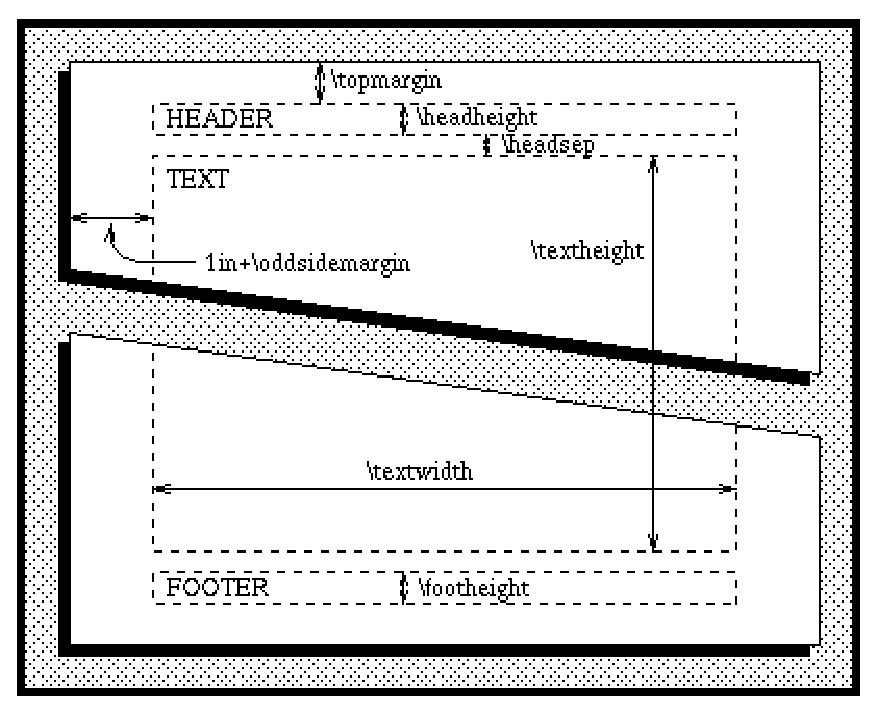
\epsfig{file=pagesetup.eps,scale=.80}
\end{center}
\label{img:margin}
\end{figure}

An author can simply set the dimensions of the document, for example, with this command:
\begin{quote}
\begin{verbatim}
\textheight 8in
\end{verbatim}
\end{quote}
Alternatively, the author can add to a length with the following:
\begin{quote}
\begin{verbatim}
\addtolength{\textheight}{2in}
\end{verbatim}
\end{quote}

Unfortunately, editing margins can become cumbersome since body text may overlap footnote text. Normally, a student will want to use one inch margins. Instead of using the aforementioned commands, I suggest using the \texttt{fullpage} package.

\subsubsection{\texttt{fullpage} Package}

Simply put, the \texttt{fullpage} package lets the author use one inch margins without manually changing them. The package is invoked with:
\begin{quote}
\begin{verbatim}
\usepackage{fullpage}
\end{verbatim}
\end{quote}
There are options available with this package, such as setting margins to 1.5cm, but this is not too helpful for school work. I suggest looking at the supplemental documents for more information. Nevertheless, I highly recommend this package for class work.

\subsection{Headers}

Headers can also be set in the preamble. To do this, a package called \texttt{fancyhdr} must be used. Load the package with the following:
\begin{quote}
\begin{verbatim}
\usepackage{fancyhdr}
\pagestyle{fancy}
\end{verbatim}
\end{quote}
The \texttt{$\backslash$pagestyle\{fancy\}} command lets \LaTeX\ know that the author wants headers. The author may omit the second line to eliminate headers.

Now that the package is loaded and active, the headers can be set. There are two sets header commands: one set is used for basic, one--sided documents; the other is generally for two--sided documents. A homogeneous set of headers can be made with three basic commands:
\begin{quote}
\begin{verbatim}
\lhead{...}
\chead{...}
\rhead{...}
\end{verbatim}
\end{quote}
These commands will make headers justified to the left, center, and right, respectively. By default, the section name and section number will appear on the left side of the header. To eliminate this, use \texttt{$\backslash$lhead\{\}} to clear the space.

Likewise, an author can move the page number with header (and footer) commands. By default, the page number will appear centered in the footer. The following will move the page number to the right side of the header:
\begin{quote}
\begin{verbatim}
\fancyhf{}
\rhead{\page}
\end{verbatim}
\end{quote}
The \texttt{$\backslash$fancyhf\{\}} will clear the header and footers, then the subsequent line will place the page in the right header.

Footer commands are very similar to header commands. Instead of, for instance, \texttt{$\backslash$rhead\{\ldots\}}, the corresponding footer command would be \texttt{$\backslash$rfoot\{\ldots\}}. To place the page number in the lower right hand side, the necessary commands would be:
\begin{quote}
\begin{verbatim}
\fancyhf{}
\rfoot{\page}
\end{verbatim}
\end{quote}

If the author is creating a two--sided document, then I suggest using different headers and footers for odd and even pages for a sophisticated look. Instead of using the previous commands, the following command is used:
\begin{quote}
$\backslash$fancyhead[\textit{option}]\{\textit{text}\}
\end{quote}
The options section is where the author declares which pages it applies to (even or odd) and which side the text should appear (left, right, or center). Table \ref{tbl:fancyhdr} list the abbreviations used for \textit{options}.
\begin{table}[!hb]\label{tbl:fancyhdr}
	\begin{center}
	\begin{tabular}{l|l} 
		\hline
		R & Right Side \\
		L & Left Side	 \\
		C & Center	   \\
		\hline
		E & Even Pages \\
		O & Odd Pages  \\
		\hline
	\end{tabular} \caption{Abbreviations for \texttt{fancyhead} command.}
	\end{center}
\end{table}

For example, placing the page number on the outside (left side for odd pages, right side for even), requires the following:
\begin{quote}
\begin{verbatim}
\fancyhf{}
\fancyhead[LO]{\page}
\fancyhead[RE]{\page}
\end{verbatim}
\end{quote}

\subsection{A Trick Using \texttt{fullpage} and \texttt{fancyhdr}}

Using a different header for odd and even pages is rather interesting. However, when using the default margins for a document, a two--sided document has different margins for odd and even pages. Odd pages have a large margin on the right, even pages have a large margin on the left. The purpose of this is to make room for binding. If you do not wish to print two--sided\footnote{Typically, printers cannot print two--sided. However, one may print odd pages only, flip the pages, then print even pages.} documents, that usually eliminates the chance of using the \texttt{$\backslash$fancyhead} command.

However, there is a way around this problem. First, load the \texttt{fullpage} package, then load the \texttt{fancyhdr} package. Since the margins on all sides of the document is the same (one inch), there will be no extra space for the binding. Thus, the author can use the \texttt{$\backslash$fancyhead} command without printing on both sides. Normally, I choose add the title to the header of the odd numbered pages and my name to the header of even numbered pages. This gives the document a very polished and professional look.

You may copy and paste the commands I've listed below:
\begin{quote}
\begin{verbatim}
\documentclass[twosided]{article}
\usepackage{fullpage}
\usepackage{fancyhdr}

\pagestyle{fancy}

\fancyhead[LO]{author's name}
\fancyhead[RE]{title}
\end{verbatim}
\end{quote}

\section{Conclusion}

Quite a bit of information was contained in this lecture. However, I suggest using the short cuts I have provided, namely, the \texttt{fullpage} package. Also, I suggest looking at the source code of this document to see how the \texttt{$\backslash$title} and \texttt{$\backslash$author} commands can be used.

\end{document}